\begin{figure}
\fontsize{12pt}{12pt}\selectfont
\resizebox{\textwidth}{!}{
\begin{tabular}{cccc}
(a) Uwaga miękka
& (b) Uwaga przestrzenna
&(c) Uwaga adaptacyjna
&(d) Uwaga  wielowarstwowa\\
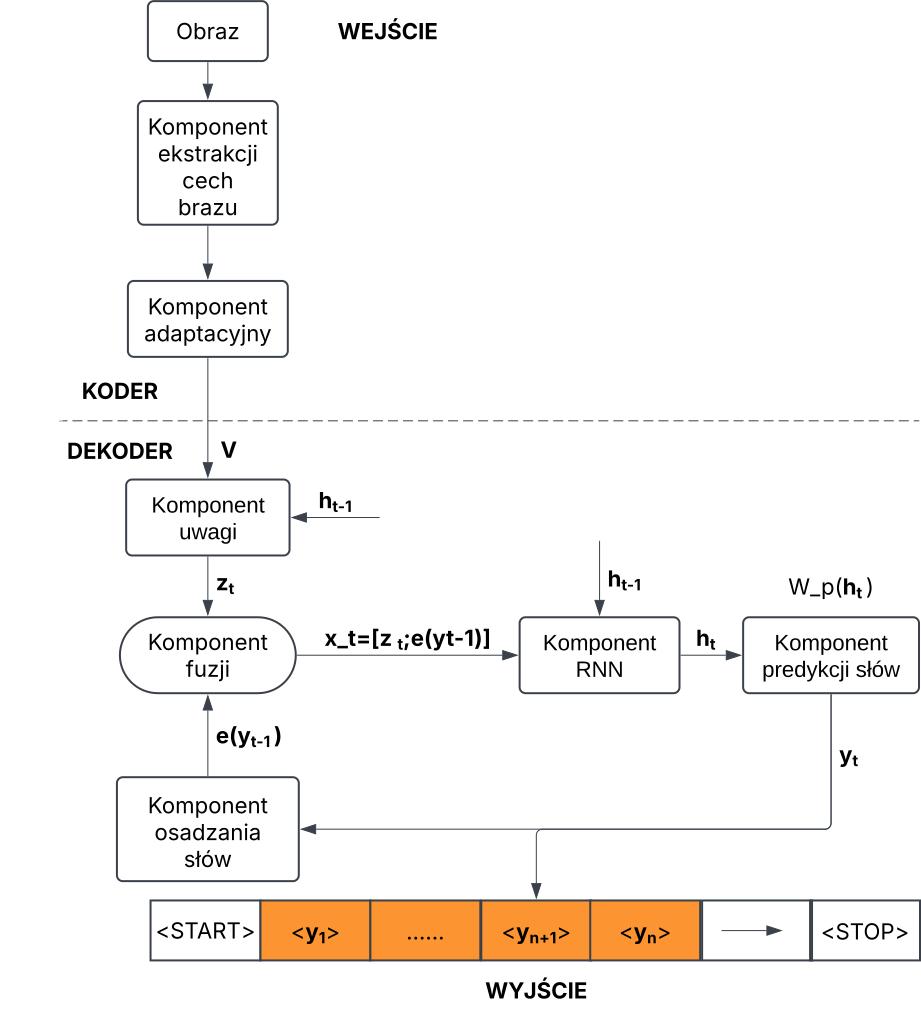
\includegraphics{wykresy/rodzaje_badanej_uwagi/uwaga_miekka.png}
&
\includegraphics{wykresy/rodzaje_badanej_uwagi/uwaga_przestrzenna.png} 
&
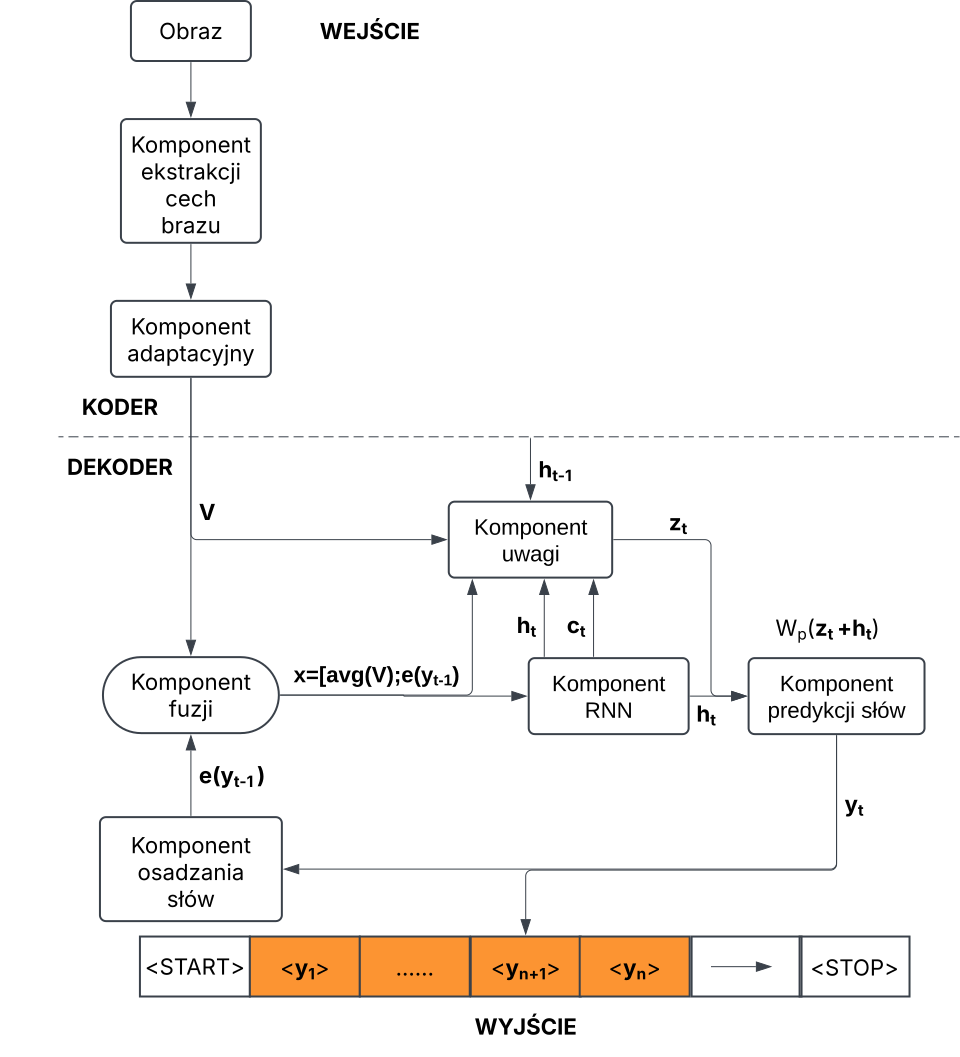
\includegraphics{wykresy/rodzaje_badanej_uwagi/uwaga_adaptacyjna.png} 
&
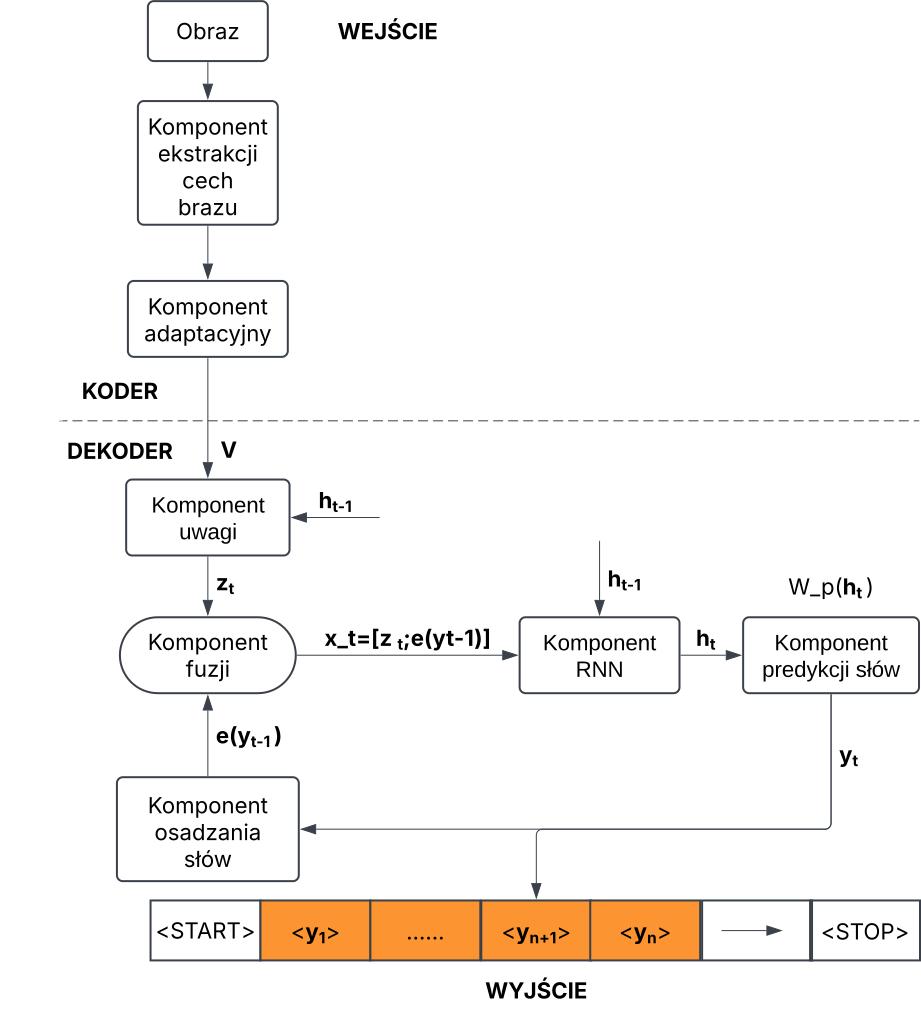
\includegraphics{wykresy/rodzaje_badanej_uwagi/uwaga_miekka.png} 

\\

\end{tabular}}
\caption{Uwaga miękka, uwaga przestrzenna, uwaga adaptacyjna, uwaga wielowarstwowa }
\label{fig:modele_jezykowe}

\end{figure}